A configuração típica do retificador trifásico com ponto médio a tiristor pode ser observada na figura \ref{ctpm}. Define-se as tensões de alimentação (tensões de fase) igualmente defasadas, i.e.,
\begin{align*}
 V_{1}(\omega{t}) &= V_{o}\sin(\omega{t}) \\
 V_{2}(\omega{t}) &= V_{o}\sin(\omega{t}-120^0) \\
 V_{3}(\omega{t}) &= V_{o}\sin(\omega{t}+120^0)
.\end{align*}
 
 \begin{figure}[h]
\center
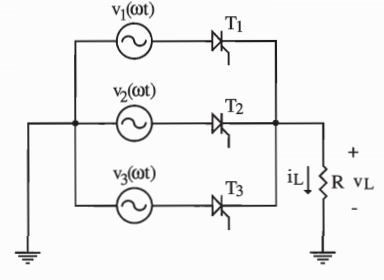
\includegraphics[scale=0.55]{imagens/circuito_trifasico_ponto_medio.png}
\caption{Circuito típico de um retificador trifásico de ponto médio a tiristor.}\label{ctpm}
\caption*{Fonte: Eletrônica de potência (2006)}
\end{figure}
 
 
A figura \ref{g1tm} ilustra a tensão na carga que possui somente componente resistivo. Veja que o ângulo de disparo $\alpha = 0$, gerando condução contínua. Na verdade, é fácil observar que isso é verdade para $\alpha < \frac{\pi}{6}$. Nesse caso, a tensão média pode ser calculada como
\begin{align*}
    V_{L,med} &= \frac{3}{2\pi}\int_{\frac{\pi}{6}+\alpha}^{\frac{5\pi}{6}+\alpha}\sqrt{2}V_{o}\sin(\omega{t})d(\omega{t}) \\
&= \frac{3\sqrt{2}V_{o}}{2\pi}[-\cos(\omega{t})]_{\pi/6+\alpha}^{5\pi/6+\alpha} \\
&= \frac{3\sqrt{2}\sqrt{3}V_{o}}{2\pi}\cos\alpha \\
&\approx 1,17\,V_{o}\cos\alpha
.\end{align*}
Veja que esse é o mesmo resultado do retificador a diodo, conforme esperado.

\begin{figure}[h]
\center
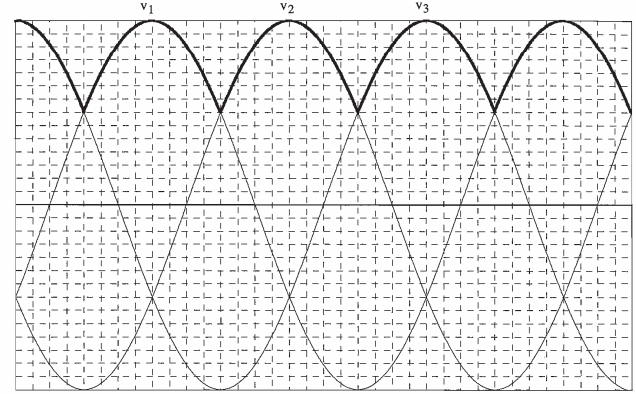
\includegraphics[scale=0.55]{imagens/grafico1_trifasico_ponto_medio_r.png}
\caption{Tensão na carga puramente resistiva para $\alpha = 0$ em um retificador trifásico de ponto médio a tiristor.}\label{g1tm} 
\caption*{Fonte: Eletrônica de potência (2006)}
\end{figure}

Para $\frac{5\pi}{6} > \alpha > \frac{\pi}{6}$, como ilustra a figura \ref{g2tm}, temos condução descontínua, ou seja, a tensão média se torna
\begin{align*}
    V_{L,med} &= \frac{3}{2\pi}\int_{\frac{\pi}{6}+\alpha}^{\pi}\sqrt{2}V_{o}\sin(\omega{t})d(\omega{t}) \\
&= \frac{3\sqrt{2}V_{o}}{2\pi}\left[-\cos\left(\omega{t}\right)\right]_{\frac{\pi}{6}+\alpha}^{\pi} \\
&= \frac{3\sqrt{2}V_{o}}{2\pi}\left[  1+\cos\left(  \frac{\pi}{6}+\alpha\right) \right]  \\
&\approx 0,675 V_{o}\left[  1+\cos\left(  \frac{\pi}{6}+\alpha \right) \right] 
.\end{align*}
Note que $\alpha = \frac{5\pi}{6} \implies V_{L,med} = 0$. O comportamento da tensão média em relação ao ângulo de disparo pode ser observado na figura \ref{g4tm}.

\begin{figure}[h]
\center
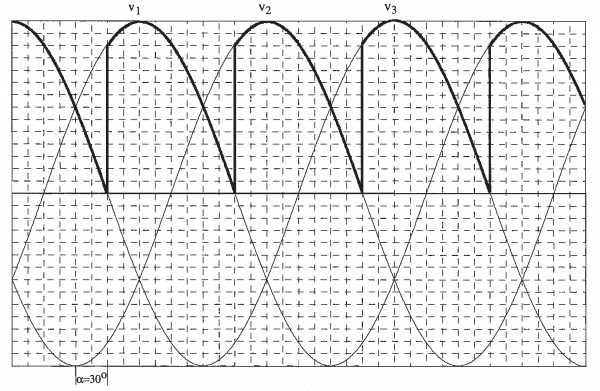
\includegraphics[width=0.45\textwidth]{imagens/grafico2_trifasico_ponto_medio_r.png}
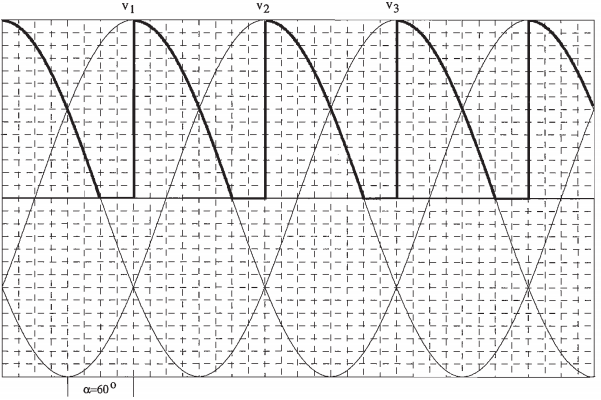
\includegraphics[width=0.45\textwidth]{imagens/grafico3_trifasico_ponto_medio_r.png}
\caption{Tensão na carga puramente resistiva para $\alpha = \frac{\pi}{6}$ (à esquerda) e $\alpha = \frac{\pi}{3}$ (à direita) em um retificador trifásico de ponto médio a tiristor.}\label{g2tm} 
\caption*{Fonte: Eletrônica de potência (2006)}
\end{figure}

\begin{figure}[h]
\center
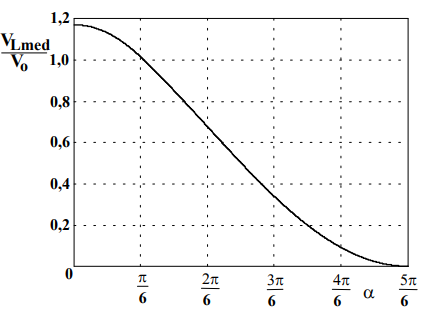
\includegraphics[scale=0.55]{imagens/grafico4_trifasico_ponto_medio_r.png}
\caption{$V_{L,med}$ em função de $\alpha$ de um retificador trifásico com ponto médio a tiristor para carga resistiva.} \label{g4tm} 
\caption*{Fonte: Eletrônica de potência (2006)}
\end{figure}

Para uma carga com componente indutivo de característica linar, a tensão média é dada por \[
V_{L,med} = 1,17V_{o}\cos\alpha
.\]
A figura \ref{g1tml} ilustra a tensão média em função de $\alpha$ para esse cenário.

\begin{figure}[h]
\center
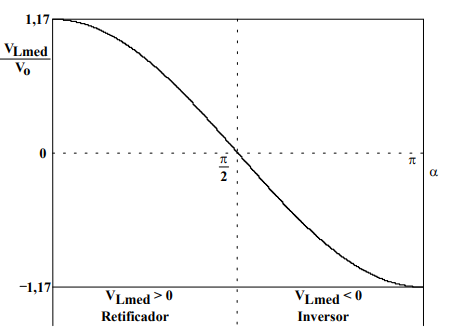
\includegraphics[scale=0.55]{imagens/grafico1_trifasico_ponto_medio_l.png}
\caption{$V_{L,med}$ em função de $\alpha$ em um retificador trifásico de ponto médio a tiristor com carga indutiva.} \label{g1tml} 
\caption*{Fonte: Eletrônica de potência (2006)}
\end{figure}

Veja que, como já visto anteriormente, essa estrutura pode operar tanto como retificador quanto como inversor. Esses dois modos de operação são visíveis na figura \ref{g2tml}.

\begin{figure}[h]
\center
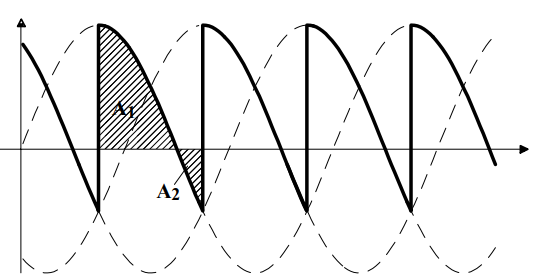
\includegraphics[scale=0.55]{imagens/grafico2_trifasico_ponto_medio_l.png}
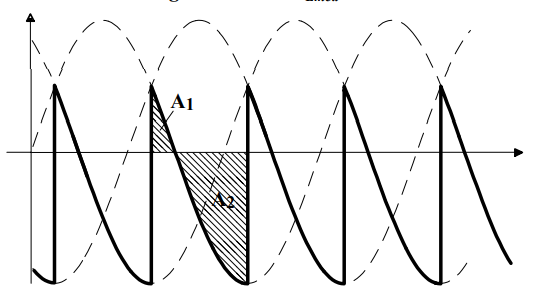
\includegraphics[scale=0.55]{imagens/grafico3_trifasico_ponto_medio_l.png}
\caption{Tensão média na carga com componente indutivo de um tiristor trifásico com ponto médio a tiristor para operação como retificador (à esquerda) e como inversor (à direita).} \label{g2tml} 
\caption*{Fonte: Eletrônica de potência (2006)}
\end{figure}

